\section{Versuchsaufbau}

\begin{figure}[H]
\begin{center}
  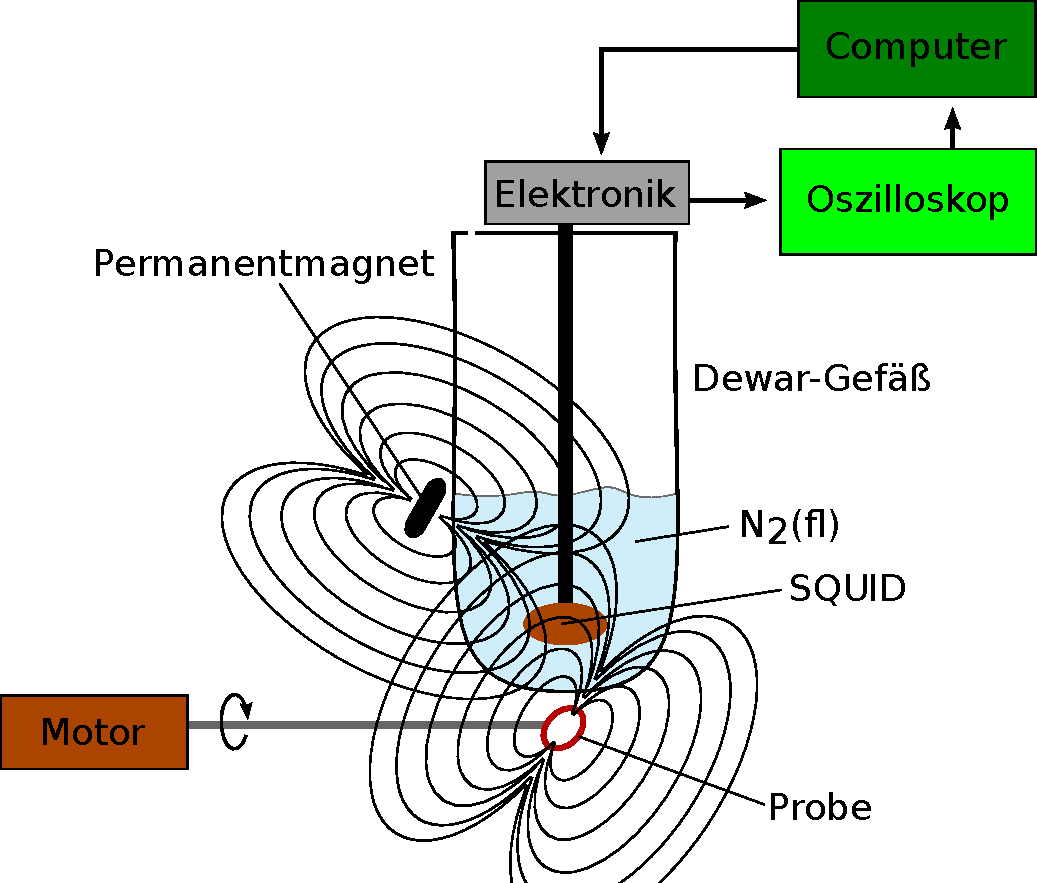
\includegraphics[width=0.8\textwidth]{../img/aufbau.pdf}
  \caption{Aufbau zur Messung kleiner Magnetfeldänderungen mit einem
  \emph{Superconducting Quantum Interference Device}.}
  \label{img:aufbau}
\end{center}
\end{figure}

\autoref{img:aufbau} zeigt den Aufbau, der für die Messungen des Magnetfelds verwendet wird.
Unter einem temperaturisolierten Behälter, der mit flüssigem Stickstoff (Temperatur 77\,K) gefüllt ist,
befindet sich eine Probe.
Die Probe wird mit einem Motor in Rotation versetzt,
so dass ein veränderliches Magnetfeld in dem Behälter erzeugt wird.
Ein weiteres, statisches Magnetfeld wird von einem beweglichen Permanentmagneten verursacht,
so dass ein während der Messung auftretender Offset (z.B. durch das Magnetfeld elektrischer Verbraucher)
kompensiert werden kann.
Eingetaucht in den Stickstoff ist das \emph{SQUID},
das von einer Elektronik über dem Behälter gesteuert und ausgelesen wird.
Die notwendigen Einstellungen der Elektronik können mit dem Computer vorgenommen werden.
Das Signal des \emph{SQUID} wird an ein Oszilloskop gesendet und
von dort weiter an einen Computer.\\
Der innere Aufbau des \emph{SQUID} ist auf \autoref{img:aufbau2} gezeigt:
Über der (magnetischen) Probe befindet sich ein supraleitender Ring, der an einer Stelle durch einen
isolierenden Josephson-Kontakt unterbrochen ist.
Von einem Schwingkreis wird mit einem Wechselstrom ein elektromagnetisches Feld erzeugt,
das den Ring durchdringt. Nimmt der Ring Energie aus diesem elektromagnetischen Feld auf,
zeigt sich dies durch eine Abnahme der Spannungsamplitude am Schwingkreis. 




\begin{figure}[H]
\begin{center}
  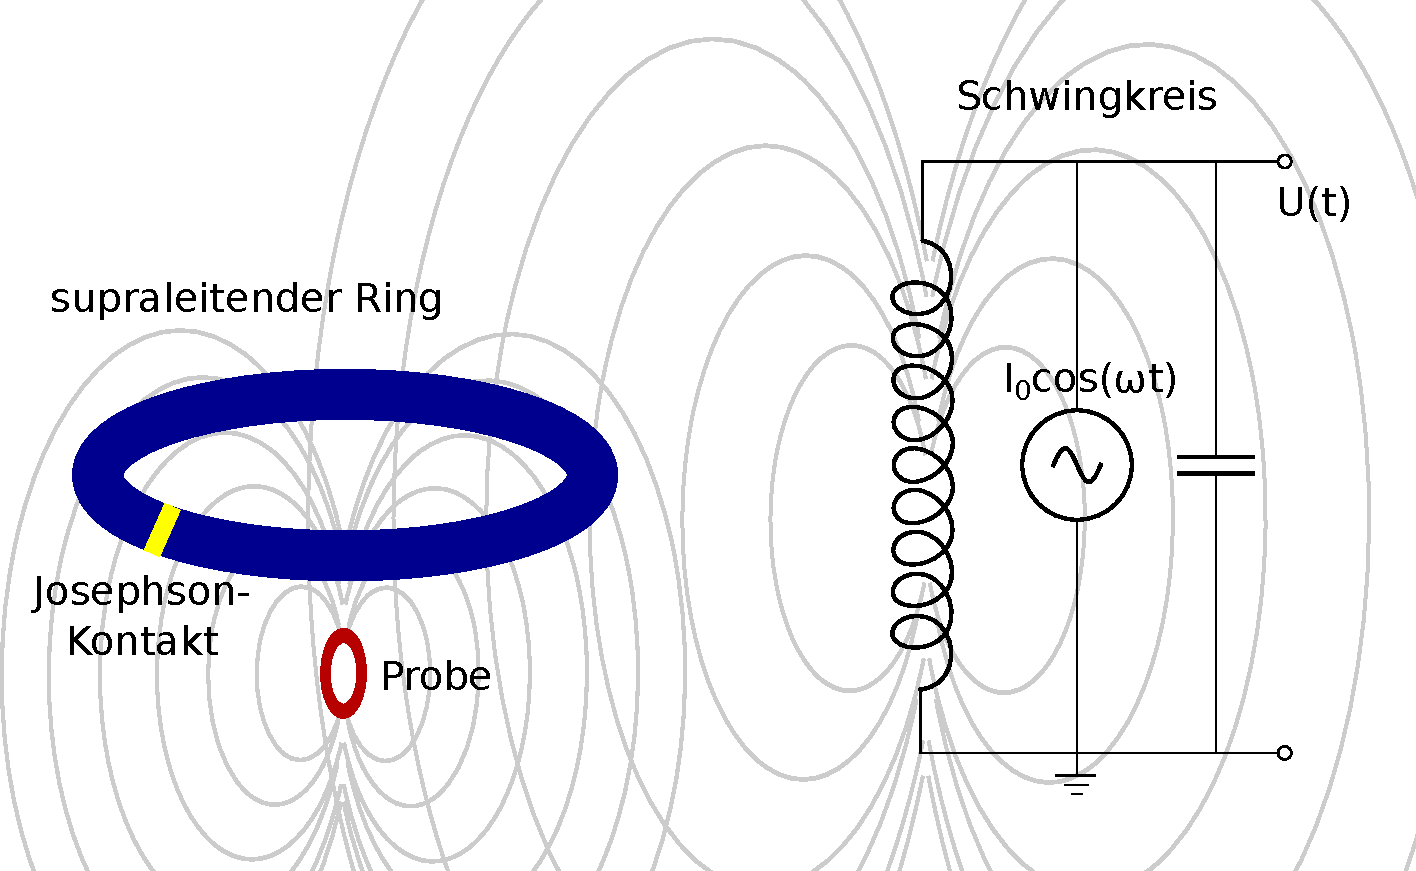
\includegraphics[width=0.7\textwidth]{../img/aufbau2.pdf}
  \caption{Aufbau des \emph{SQUID}: Schwingkreis zur Erzeugung eines elektromagnetischen Wechselfelds
  an einem supraleitenden Ring und zur Messung der Energieaufnahme bei Verlust seiner Supraleitfähigkeit.}
  \label{img:aufbau2}
\end{center}
\end{figure}